\documentclass{lib/myskripsi}


\usepackage{blindtext}
\usepackage{longtable}

% \usepackage{showframe}
% \usepackage[compact]{titlesec}

%=============================================================================
% Definisi Data Peneliti, Judul, Pembimbing dan Penguji
%-----------------------------------------------------------------------------
\titleind{IMPLEMENTASI FILTER SPASIAL LINEAR PADA VIDEO \textit{STREAM} MENGGUNAKAN \textit{FPGA HARDWARE ACCELERATOR}}

\fullname{SULAEMAN}
\idnum{H131 16 002}

% \examdate{\hspace{0.4cm} Mei 2021}

\degree{Sarjana Sains}
\yearsubmit{2021}
\program{Ilmu Komputer}
\dept{Matematika}
\faculty{Fakultas Matematika dan Ilmu Pengetahuan Alam}

\firstsupervisor{Dr. Eng. Armin Lawi, S.Si., M.Eng.}
\firstsupervisorNIP{94199834743819}
\secondsupervisor{Supri Bin Hj Amir, S.Si., M.Eng.}
\secondsupervisorNIP{196402171991031004}
\firstexaminer{ Dr. Hendra, S.Si., M.Kom.}
\secondexaminer{ Nur Hilal A Syahrir, S.Si., M.Si.}
%-----------------------------------------------------------------------------
% End Definisi Data Peneliti, Judul, Pembimbing dan Penguji
%=============================================================================

\begin{document}
    \noindent
    \textit{Seminar II}
    \coverproposal
    \pagenumbering{roman}

    %=============================================================================
    % Daftar isi, daftar gambar, daftar tabel
    %-----------------------------------------------------------------------------
    \tableofcontents
    \addcontentsline{toc}{chapter}{DAFTAR ISI}
    \newpage

    \listoftables
    \addcontentsline{toc}{chapter}{DAFTAR TABEL}
    \newpage

    \listoffigures
    \addcontentsline{toc}{chapter}{DAFTAR GAMBAR}
    \newpage
    %-----------------------------------------------------------------------------
    % End Daftar isi, daftar gambar, daftar tabel
    %=============================================================================

    \pagebreak
    \pagenumbering{arabic}

    %=============================================================================
    % Daftar masukan untuk Bab
    %-----------------------------------------------------------------------------
    \chapter{PENDAHULUAN}

\section{Latar Belakang}

% perlu diperbaiki 

% Tentang Citra digital
Citra digital merupakan citra yang dihasilkan dari pengolahan secara digital dengan merepresentasikan citra secara numerik dengan nilai-nilai diskrit. Suatu citra digital dapat direpresentasikan dalam bentuk matriks dengan fungsi \textit{f(x,y)} yang terdiri dari M kolom dan N baris. Perpotongan antara baris dan kolom disebut sebagai piksel \cite{book:gonzalez}. 

% Pengolahan Citra digital
Pengolahan citra digital merupakan proses mengolah piksel di dalam citra secara digital untuk tujuan tertentu. Berdasarkan tingkat pemrosesannya pengolahan citra digital dikelompokkan menjadi tiga kategori, yaitu: \textit{low-level}, \textit{mid-level} dan pemrosesan \textit{high-level}. Pemrosesan \textit{low-level} dilakukan dengan operasi primitif seperti \textit{image preprocessing} untuk mengurangi derau (\textit{noise}), memperbaiki kontras citra dan mempertajam citra (\textit{sharpening}). Pemrosesan \textit{mid-level} melibatkan tugas-tugas seperti segmentasi atau mempartisi gambar menjadi beberapa bagian atau objek, deskripsi objek untuk dilakukan pemrosesan lanjutan, dan klasifikasi objek yang terdapat dalam citra digital. Pemrosesan \textit{high-level} merupakan proses tingkat lanjut dari dua proses sebelumnya, dilakukan untuk mendapat informasi lebih yang terkandung dalam citra seperti \textit{pattern recognition}, \textit{template matching}, \textit{image analysis} dan sebagainya \cite{book:gonzalez}.


% Filter Spasial
Konsep filter spasial pada pengolahan citra digital berasal dari penerapan transformasi Fourier untuk pemrosesan sinyal pada domain frekuensi. Istilah filter spasial ini digunakan untuk membedakan proses ini dengan filter pada domain frequensi. Proses filter dilakukan dengan cara menggeser filter kernel dari titik ke titik dalam citra digital. Istilah \textit{mask}, \textit{kernel}, \textit{template}, dan \textit{window} merupakan isitilah yang sama dan sering digunakan dalam pengolahan citra digital. Dalam penelitian ini peneliti menggunakan istilah kernel untuk istilah tersebut. Konsep filter spasial linear mirip seperti konsep konvolusi pada domain frekuensi, dengan alasan tersebut filter spasial linear biasa disebut juga konvolusi sebuah kernel dengan citra digital \cite{book:gonzalez}. Proses filter dalam pengolahan citra digital dilakukan dengan memanipulasi sebuah citra menggunakan kernel untuk menghasilkan citra yang baru, sehingga dengan kernel yang berbeda maka citra hasil yang didapat juga akan berbeda. 


% Stream Video adalah
Video \textit{stream} dapat dipandang sebagai serangkaian citra digital berturut-turut \cite{thesis:jin}. Berbeda dengan format video lainya, video \textit{stream} ini tidak disimpan pada media penyimpanan sebagai file video melainkan setiap \textit{frame} langsung disalurkan dari sumber (\textit{source}) ke penerima, dalam hal ini FPGA. Dengan menganggap video \textit{stream} adalah kumpulan citra digital (\textit{frame}) maka dapat dilakukan metode pengolahan seperti pada citra digital, termasuk filter spasial. 

Frame per second (\textit{fps}) atau \textit{frame rate} adalah banyaknya \textit{frame} yang ditampilkan per detik. Semakin tinggi \textit{fps} sebuah video maka semakin baik pula gerakan yang dapat ditampilkan karena dibentuk dari \textit{frame} yang lebih banyak. Namun dengan jumlah \textit{frame} yang lebih besar tentu dibutuhkan juga \textit{resource} yang lebih besar dalam pengolahan video tersebut \cite{pdf:marcin}. 
% Dalam penelitian ini video stream yang digunakan dibatasi 30 \textit{fps} saja dengan resolusi 720p.




% FPGA Xilinx PYNQ-Z2 adalah FPGA \textit{Board} yang digunakan pada penelitian ini secara \textit{official} dapat menerima input video \textit{stream} dengan resolusi 720p. Setiap \textit{frame} yang diterima dari \textit{source} akan dilakukan proses filter spasial, kemudian hasilnya disalurkan melalui HDMI output untuk kemudian ditampilkan. Video hasil filter spasial yang ditampilkan akan mengalami penurunan \textit{fps}, hal ini disebabkan adanya penambahan jeda waktu komputasi untuk proses filter yang dilakukan pada setiap \textit{frame}. Pada kesempatan ini peneliti ingin melakukan "Implementasi Filter Spasial Linear pada Video \textit{Stream} menggunakan FPGA \textit{Hardware Accelerator}".


Untuk meningkatkan kinerja dan efisiensi energi dari sebuah program, berbagai jenis akselerator telah dikembangkan, salah satu diantaranya yaitu FPGA \cite{lb:cong}. \textit{Field Programmable Gate Arrays} atau FPGA adalah perangkat semikonduktor yang berbasis \textit{matriks configurable logic block} (CLBs) yang terhubung melalui interkoneksi yang dapat diprogram. FPGA dapat diprogram ulang dengan aplikasi atau fungsi yang diinginkan setelah \textit{manufacturing}. Fitur ini yang membedakan FPGA dengan \textit{Application Specific Integrated Circuits} (ASICs), yang dibuat khusus untuk tugas tertentu saja \cite{XILINX}.

FPGA telah menunjukkan kinerja yang sangat tinggi di dalam banyak aplikasi dalam pemrosesan citra. Namun CPU dan CPU terbaru memiliki potensi kinerja tinggi untuk masalah-masalah tersebut. CPU terbaru mendukung \textit{multi-core}, dimana masing-masing \textit{core} mendukung SIMD (\textit{Single Instruction, Multiple Data}) yang telah dikembangkan dan dijalankan hingga 16 operasi pada 128 bit data dalam satu \textit{clock cycle}. GPU terbaru mendukung sejumlah besar \textit{core} yang berjalan secara paralel, dan kinerja puncaknya mengungguli CPU \cite{lb:asano}.

\pagebreak

Paralelisme dalam SIMD pada CPU terbatas, tetapi frekuensi operasional CPU sangatlah tinggi, dan CPU diharapkan dapat menunjukkan kinerja yang tinggi dalam aplikasi yang dimana \textit{cache memory} berjalan dengan baik. Ukuran \textit{cache memory} cukup besar untuk menyimpan seluruh citra di banyak aplikasi pemrosesan citra, dan CPU dapat menjalankan algoritma yang sama dengan FPGA meskipun \textit{bandwith memory} yang dibutuhkan tinggi \cite{lb:asano}.

Frekuensi operasional GPU lebih cepat dibandingkan dengan FPGA, namun sedikit lebih lambat dibandingkan dengan CPU. Akan tetapi, GPU mendukung banyak \textit{core} yang berjalan secara paralel sehingga kinerja puncaknya mengungguli CPU. Namun \textit{core}-nya dikelompokkan, dan transfer data antara kelompok sangatlah lambat. Selain itu, ukuran \textit{local memory} yang disediakan masing-masing kelompok sangat kecil. Karena keterbatasan ini, GPU tidak dapat menjalankan algoritma yang sama seperti FPGA dalam beberapa masalah aplikasi \cite{lb:asano}.

Pada FPGA terdahulu tidak terdapat prosesor untuk menjalankan \textit{software} apapun, sehingga ketika ingin mengimplementasikan aplikasi haruslah merancang sirkuit dari awal. Sebagian besar FPGA sekarang telah dirangkai dengan prosesor dalam satu \textit{board}, sering disebut sebagai FPGA Development Board. Xilinx PYNQ-Z2 dibangun dari prosesor ARM Cortex-A9, sehingga dapat menjalankan beberapa \textit{software} seperti \textit{python} tanpa harus merancang sirkuitnya dari awal. Akan tetapi, kinerja yang dimiliki oleh prosesor ARM pada FPGA Development Board tentu berbeda dengan kinerja fungsi arsitektur FPGA itu sendiri sehingga dapat dikaji lebih dalam mengenai perbandingan kinerja dari keduanya.

Berdasarkan uraian permasalahan di atas, peneliti ingin melakukan penelitian dengan judul "Implementasi Filter Spasial Linear pada Video \textit{Stream} menggunakan FPGA \textit{Hardware Accelerator}" untuk menunjukkan kinerja dari prosesor ARM dan FPGA pada Xilinx PYNQ-Z2 FPGA Development Board.

\pagebreak

\section{Rumusan Masalah}
Adapun rumusan masalah dalam penelitian ini yaitu:
\begin{enumerate}[topsep=0pt,itemsep=0pt,partopsep=0pt, parsep=0pt]
    \item Bagaimana cara implementasi fiter spasial linear pada video \textit{stream} menggunakan FPGA? 
    \item Bagaimana kinerja FPGA dalam mengimplementasikan fiter spasial linear pada video \textit{stream}? 
\end{enumerate}

\section{Tujuan Penelitian}
Adapun tujuan dari penelitian ini yaitu:
\begin{enumerate}[topsep=0pt,itemsep=0pt,partopsep=0pt, parsep=0pt]
    \item Mampu melakukan implementasi fiter spasial linear pada video \textit{stream} menggunakan FPGA.
    \item Mengetahui kinerja FPGA dalam mengimplementasikan fiter spasial linear pada video \textit{stream}.
\end{enumerate}


\section{Batasan Masalah}
Berikut ini merupakan beberapa batasan dalam penelitian ini.
\begin{enumerate}[topsep=0pt,itemsep=0pt,partopsep=0pt, parsep=0pt]
    \item Filter kernel yang digunakan berukuran 3x3.
    \item Video \textit{stream} yang digunakan dalam penelitian ini beresolusi 720p.
    \item Setiap frame dari video \textit{stream} diubah menjadi citra grayscale sebelum dilakukan penerapan filter spasial.
    \item FPGA \textit{Board} yang digunakan adalah Xilinx PYNQ-Z2 dengan processor 650MHz dual-core ARM Cortex-A9.
\end{enumerate}

\section{Manfaat Penelitian}
Hasil dari penelitian ini diharapkan dapat memberikan pemahaman tentang penerapan filter spasial pada video \textit{stream} dengan FPGA Development Board. Selain itu, penelitian ini juga diharapkan dapat menjadi rujukan untuk melihat kinerja FPGA PYNQ-Z2 dalam mengimplementasikan filter spasial linear pada video \textit{stream}.

    
\chapter{TINJAUAN PUSTAKA}


\section{Landasan Teori}

\subsection{Citra Digital}
Citra digital dapat didefinisikan sebagai fungsi \textit{f(x,y)} berukuran M baris dan N kolom, dengan \textit{x} dan \textit{y} adalah kordinat spasial, dan amplitudo \textit{f} di titik kordinat (x,y) dinamakan intensitas atau tingkat keabuan dari citra pada citra tersebut \thecite{book:darma}. Pada umumnya warna dasar dalam citra RGB menggunakan penyimpanan 8 bit untuk menyimpan data warna, yang berarti setiap warna mempunyai gradasi sebanyak 255 warna . Dewasa ini, citra digital dapat menggunakan 16 bit untuk menyimpan data warna dasarnya, hal ini menyebabkan semakin banyak gradasi warnanya sehingga citra yang dihasilkan memiliki tingkat warna yang jauh lebih banyak. Namun tentu saja hal ini mengakibatkan ukuran file citra digital yang dihasilkan juga menjadi semakin besar walaupun dengan ukuran yang sama. Berdasarkan jenis warnanya citra digital dibagi menjadi 3 jenis:

\begin{enumerate} [label=\textbf{\alph*.}]
    \item \textbf{Citra Biner (monokrom)} \\ 
    Citra biner hanya memiliki dua warna saja, yaitu hitam dan putih. Warna hitam direpresentasikan dengan 1 dan warna putih direpresentasikan dengan 0. Dibutuhkan 1 bit di memori untuk menyimpan warna ini. Contoh citra biner dapat dilihat pada gambar ~\ref{fig:jenis-citra}(a).
    \item \textbf{Citra Grayscale} \\ 
    Banyaknya warna tergantung pada jumlah bit yang disediakan di memori untuk menampung kebutuhan warna ini. Citra \textit{grayscale} 2 bit memiliki 4 gradasi warna, citra \textit{grayscale} 3 bit memiliki 8 gradasi warna, dan seterusnya. Semakin besar jumlah bit warna yang disediakan di memori, semakin banyak dan semakin halus gradasi warna yang terbentuk. Pada umumnya citra digital \textit{grayscale} menggunakan 8 bit memori dengan derajat keabuan dari 0 sampai 255. Contoh citra \textit{grayscale} dapat dilihat pada gambar ~\ref{fig:jenis-citra}(b).
    \item \textbf{Citra Warna} \\ 
    Setiap piksel pada citra warna mewakili warna yang merupakan kombinasi dari tiga warna dasar (RGB = Red Green Blue). Setiap warna dasar menggunakan penyimpanan 8 bit, yang berarti setiap warna mempunyai gradasi sebanyak 255 warna. Berarti setiap piksel mempunyai kombinasi warna sebanyak 255 x 255 x 255 =16 juta warna lebih. Contoh citra warna dapat dilihat pada gambar ~\ref{fig:jenis-citra}(c).
\end{enumerate}

\begin{afigure}
    \includegraphics[width=0.85\textwidth, center]{images/jenis-jenis-citra.png}
    \caption{(a) Contoh citra biner, (b) contoh citra grayscale, (c) contoh citra warna.}
    \label{fig:jenis-citra}
\end{afigure}


\subsection{Pengolahan Citra Digital}
Pengolahan citra digital merupakan proses mengolah piksel-piksel di dalam citra secara digital untuk tujuan tertentu. Berdasarkan tingkat pemrosesannya pengolahan citra digital dikelompokkan menjadi tiga kategori, yaitu: \textit{low-level}, \textit{mid-level} dan pemrosesan \textit{high-level}. Pemrosesan \textit{low-level} dilakukan dengan operasi primitif seperti \textit{image preprocessing} untuk mengurangi derau (\textit{noise}), memperbaiki kontras citra dan mempertajam citra (\textit{sharpening}). Karakteristik dari pemrosesan \textit{low-level} yaitu keluaran atau hasil dari pemrosesannya berupa citra digital. Pemrosesan \textit{mid-level} melibatkan tugas-tugas seperti segmentasi (mempartisi gambar menjadi beberapa bagian atau objek), deskripsi objek untuk dilakukan pemrosesan lanjutan, dan klasifikasi objek dalam citra digital. Karakteristik dari pemrosesan \textit{mid-level} yaitu keluaran atau hasilnya berupa atribut atau fitur seperti, kontur, tepi, atau objek yang terdapat dalam citra tersebut. Pemrosesan \textit{high-level} merupakan proses tingkat lanjut dari dua proses sebelumnya, dilakukan untuk mendapat informasi lebih yang terkandung dalam citra \thecite{book:gonzalez}.


Berdasarkan tujuannya pengolahan citra juga dapat dibagi menjadi beberapa bagian yaitu: \textit{image enhancement}, \textit{image restoration}, \textit{image analysis} dan \textit{image compression} \thecite{book:dasilva}.

\begin{enumerate} [label=\textbf{\alph*.}]
    \item \textbf{Image Enhancement} \\ 
    \textit{Image Enhancement} adalah metode pengolahan citra digital untuk membuat citra tampak lebih baik atau dilakukan peningkatan untuk analisis tertentu. Namun hal ini dapat menyebabkan pengorbanan aspek lain dari citra tersebut. Penerapan filter, penghalusan citra, memperbaiki kontras dan morfologi citra adalah contoh \textit{image enhancement}. 
    \item \textbf{Image Restoration} \\ 
    \textit{Image restoration} adalah metode pengolahan citra untuk memulihkan citra dari penurunan kualitas atau citra yang rusak karena derau (\textit{noise}). Pada dasarnya metode ini berbeda dengan \textit{image enhancement} yang berkaitan dengan ekstraksi fitur pada citra. 
    \item \textbf{Image Analysis} \\ 
    \textit{Image analysis} adalah metode pengolahan citra untuk menghitung besaran kuantitatif dari citra untuk menghasilkan deskripsinya. Metode ini dilakukan dengan mengekstraksi ciri-ciri tertentu yang membantu dalam identifikasi objek.
    \item \textbf{Image Compression} \\ 
    Metode ini dilakukan agar citra dapat direpresentasikan dalam bentuk yang lebih kompak sehingga memerlukan memori yang lebih sedikit. Metode ini dapat dilakukan dengan mengurangi redundansi dari data-data yang terdapat dalam citra sehingga dapat disimpan atau ditransmisikan secara efisien.
\end{enumerate}

\subsection{Filter Spasial}
Konsep filter spasial pada pengolahan citra digital berasal dari penerapan transformasi Fourier untuk pemrosesan sinyal pada domain frekuensi. Istilah filter spasial ini digunakan untuk membedakan proses ini dengan filter pada domain frequensi. Proses filter dilakukan dengan cara menggeser filter kernel dari titik ke titik dalam citra digital. Istilah \textit{mask}, \textit{kernel}, \textit{template}, dan \textit{window} merupakan isitilah yang sama dan sering digunakan dalam pengolahan citra digital \thecite{book:gonzalez}. Dalam penelitian ini penulis menggunakan istilah kernel untuk istilah tersebut.

Proses filter dalam pengolahan citra digital dilakukan dengan memanipulasi sebuah citra menggunakan kernel untuk menghasilkan citra yang baru, sehingga dengan kernel yang berbeda maka citra hasil yang didapat juga akan berbeda. 


\subsubsection{Operator Linear dan Non-linear}
Didefinisikan H sebuah operator dengan \textit{input} dan \textit{output} adalah citra digital. H dikatakan operator linear jika untuk untuk sembarang gambar \textit{f} dan \textit{g}, dan untuk sembarang skalar a dan b berkalu,
\begin{equation}
    \label{eq:linearity-operator}
    H(af + bg) = aH(f) + bH(g)
\end{equation}

Dengan kata lain hasil dari operator linear dengan jumlahan dua buah citra (yang telah dikali dengan konstanta a dan b) identik dengan hasil operator linear pada masing-masing gambar, dikali dengan konstanta yang sama, kemudian hasilnya dijumlahkan. Sebagai contoh, sebuah operator dengan fungsi yang menjumlahkan K citra adalah operator linear. Operator yang menghitung nilai mutlak dari perbedaan dua gambar adalah tidak linear. Operator yang tidak memenuhi persamaan (\ref{eq:linearity-operator}) dikatakan non-linear \thecite{book:gonzalez}.


\subsection{Kernel}

\subsubsection{Average Blur}
\textit{Average blur} atau biasa juga disebut \textit{box filter} adalah salah satu filter yang digunakan untuk menghaluskan citra dan mengurangi derau. Secara sederhana nilai sebuah piksel yang baru adalah nilai rata-rata dari nilai piksel tersebut dengan nilai piksel tetangganya \thecite{pdf:marcin}. Berikut kernel \textit{Average blur} yang digunakan dalam penelitian ini:
\begin{equation}
    \label{kernel:average}
    \frac{1}{9} \left[
    \begin{matrix}
        1 & 1 & 1 \\
        1 & 1 & 1 \\
        1 & 1 & 1
    \end{matrix}
    \right]
\end{equation}

\subsubsection{Gaussian Blur}
Filter ini juga digunakan untuk menghaluskan citra dan mengurangi derau. Idenya mirip seperti \textit{Average blur}, nilai piksel yang baru dibentuk dari nilai piksel tetangganya, tepai dengan memberikan bobot yang lebih kuat pada nilai pikselnya sendiri diikuti dengan bobot yang lebih rendah pada piksel atas, bawah dan sampingnya \thecite{soa:dmitry}. Berikut kernel gaussian blur filter yang digunakan dalam penelitian ini:
\begin{equation}
    \label{kernel:gaussianblur}
    \frac{1}{16}
    \left[
    \begin{matrix}
        1 & 2 & 1 \\
        2 & 4 & 2 \\
        1 & 2 & 1
    \end{matrix}
    \right]
\end{equation}

\subsubsection{Sobel}
Filter Sobel termasuk \textit{high-pass} filter yang umum digunakan untuk deteksi tepi pada citra. Sobel memiliki dua kernel untuk deteksi tepi yaitu kernel sobel vertikal untuk mendeteksi tepi secara vertikal dan kernel sobel horizontal yang mendeteksi tepi secara horizontal \thecite{pdf:marcin}. Berikut kernel Sobel vertikal dan horizontal yang digunakan dalam penelitian ini:
\begin{equation}
    \label{kernel:sobel}
    \left[
    \begin{matrix}
        1 & 0 & -1 \\
        2 & 0 & -2 \\
        1 & 0 & -1
    \end{matrix}
    \right]
    \hspace{2cm}
    \left[
        \begin{matrix}
        1 & 2 & 1 \\
        0 & 0 & 0 \\
        -1 & -2 & -1
    \end{matrix}
    \right]
\end{equation}

\subsubsection{Laplacian}
Filter ini dapat digunakan untuk deteksi tepi pada citra karena sifatnya yang sensitif dengan perubahan intensitas yang cepat \thecite{pdf:jingbo}. Tidak seperti Sobel yang menggunakan dua kernel untuk mendeteksi tepi secara vertikal dan horizontal, disini hanya digunakan sebuah kernel yang dapat digunakan untuk deteksi tepi secara vertikal dan horizontal sekaligus. Berikut kernel Laplacian yang digunakan dalam penelitian ini:
\begin{equation}
    \label{kernel:laplacian}
    \left[
    \begin{matrix}
        0 & 1 & 0 \\
        1 & -4 & 1 \\
        0 & 1 & 0
    \end{matrix}
    \right]
\end{equation}

\subsubsection{Sharpening}
Sharpening filter digunakan untuk memperjelas detail halus dalam citra atau untuk meningkatkan detail pada citra yang \textit{blur}, baik karena kesalahan ataupun karena efek dari metode akuisisi citra tertentu \thecite{pdf:ching}. Berikut kernel untuk filter \textit{sharpening} yang digunakan dalam penelitian ini:
\begin{equation}
    \label{kernel:sharpen}
    \left[
    \begin{matrix}
        -1 & -1 & -1 \\
        -1 & 9 & -1 \\
        -1 & -1 & -1
    \end{matrix}
    \right]
\end{equation}


\subsection{Konvolusi}
Konsep filter spasial linear mirip seperti konsep konvolusi pada domain frekuensi, dengan alasan tersebut filter spasial linear biasa disebut juga konvolusi sebuah kernel dengan citra digital \thecite{book:gonzalez}. Konvolusi pada fungsi \textit{f(x)} dan \textit{g(x)} didefinisikan sebagi berikut:
\begin{equation}
    \label{eq:conv1}
    \begin{split}
        h(x) = f(x) * g(x) = \int_{-\infty}^{\infty} f(a) g(x-a) da
    \end{split}
\end{equation}
dimana tanda * menyatakan operator konvolusi, dan peubah a adalah peubah bantu. Untuk fungsi diskrit, konvolusi didefinisikan sebagai berikut:
\begin{equation}
    \label{eq:conv2}
    \begin{split}
         h(x) = f(x) * g(x) = \sum_{a=-\infty}^{\infty} f(a)g(x-a)
    \end{split}
\end{equation}

Pada operasi konvolusi diatas, \textit{g(x)} disebut kernel konvolusi atau filter kernel. Kernel \textit{g(x)} dioperasikan secara bergeser pada sinyal masukan \textit{f(x)}. Jumlah perkalian kedua fungsi pada setiap titik merupakan hasil konvolusi yang dinyatakan dengan keluaran \textit{h(x)} \thecite{book:munir}. 

Pada gambar (\ref{fig:conv3}) diilustrasikan bagaimana proses konvolusi pada citra digital yang direpresentasikan dalam bentuk matriks. Operasi konvolusi dilakukan pada matriks input berukuran 6x6 dengan filter berukuran 3x3. Hasil konvolusinya ditampilkan pada matriks \textit{result}.
\begin{afigure}
    \includegraphics[width=0.85\textwidth, center]{images/convolution-operation.png}
    \caption{Ilustrasi konvolusi pada citra. Sumber: https://indoml.com}
    \label{fig:conv3}
\end{afigure}

Jika hasil konvolusi menghasilkan nilai piksel negatif, maka nilai tersebut dijadikan 0, sebaliknya jika hasil konvolusi menghasilkan nilai piksel yang melebihi nilai keabuan maksimum, maka nilai tersebut dijadikan ke nilai keabuan maksimum \thecite{book:sutoyo}.
% masalah padding
 

\subsection{Video Streaming}
Video stream dapat dipandang sebagai serangkaian citra digital berturut-turut \thecite{thesis:jin}. Berbeda dengan format video lainya, video stream ini tidak disimpan pada media penyimpanan sebagai file video melainkan langsung disalurkan setiap framenya dari sumber (\textit{source}) ke penerima, dalam hal ini FPGA.  Dengan menganggap Video stream adalah kumpulan citra digital (frame) maka dapat dilakukan metode pengolahan seperti pada citra digital, termasuk penerapan filter spasial. 


\subsection{FPGA}
\textit{Field Programmable Gate Arrays} atau FPGA adalah perangkat semikonduktor yang berbasis \textit{matriks configurable logic block} (CLBs) yang terhubung melalui interkoneksi yang dapat diprogram. FPGA dapat diprogram ulang ke aplikasi atau fungsi yang diinginkan setelah \textit{manufacturing}. Fitur ini yang membedakan FPGA dengan \textit{Application Specific Integrated Circuits} (ASICs), yang dibuat khusus untuk tugas tertentu saja \thecite{XILINX}.

Sebuah \textit{microprocessor} menerima instruksi berupa kode 1 atau 0, kode-kode ini selanjutnya diinterpretasikan oleh komputer untuk menjalankan perintah yang diberikan. \textit{Microprocessor} ini membutuhkan intruksi berupa kode secara terus menerus untuk menjalankan fungsinya. Sedangkan pada FPGA hanya dibutuhkan sekali konfigurasi \textit{chip} setiap kali dinyalakan. Membuat atau mengunduh \textit{bitstream} yang menentukan fungsi logika dilakukan oleh \textit{logic elements} (LEs), sebuah sirkuit dapat dibuat dengan mengabungkan beberapa LEs menjadi satu kesatuan. Setelah \textit{bitstream} dipasang, FPGA tidak perlu lagi membaca instruksi berupa 1 dan 0, berbeda dengan \textit{microprocessor} yang selalu membutuhkan instruksi \thecite{pdf:cheung}. Secara tradisional, untuk membuat sebuah desain FPGA, aplikasi dideskripsikan menggunakan \textit{Hardware Description Language} (HDL) seperti Verilog atau VHDL sehingga menghasilkan sebuah \textit{bitstream} FPGA. 

\begin{afigure}
    \includegraphics[width=12cm, center]{images/fpga-structure.jpeg}
    \caption{Struktur FPGA.}
    \label{fig:fpga-structure}
\end{afigure}

\subsubsection{FPGA Development Board}
Pada FPGA terdahulu tidak terdapat \textit{processor} (CPU) untuk menjalankan software apapun, sehingga ketika ingin mengimplementasikan aplikasi haruslah merancang sirkuit dari awal, seperti mengonfigurasi FPGA sesederhana gerbang logika OR atau serumit \textit{multi-core processor} \thecite{site:biswas}. Dewasa ini telah dikembangkan FPGA \textit{Develepment Board} atau biasa disebut juga FPGA \textit{Board} yaitu teknologi FPGA yang dirangkai dalam sebuah \textit{board} dan dilengkapi dengan \textit{microprocessor} dan beberapa \textit{interface} \textit{IO} untuk menjankan tugas tertenu. Umumnya FPGA \textit{Board} telah dilengkapi dengan interface untuk mengakses dan menerapkan desain sirkuitnya. Xilinx, Altera dan Intel adalah produsen FPGA \textit{Board} yang terkenal. FPGA \textit{Board} yang digunakan dalam penelitian ini yaitu Xilinx PYNQ-Z2 dengan Jupyter Notebook sebagai \textit{interface} untuk mengakses dan menjalankan program pada penelitian ini. Bentuk FPGA \textit{Board} Xilinx PYNQ-Z2 dapat dilihat pada gambar (\ref{fig:pynq-z2})

\begin{afigure}
    \includegraphics[width=7cm, center]{images/pynq-z2.jpeg}
    \caption{FPGA Board Xilinx PYNQ-Z2.}
    \label{fig:pynq-z2}
\end{afigure}


\subsection{Evaluasi Performa}

\subsubsection{Waktu Komputasi}
\thecite{pdf:chang}

\subsubsection{Frame Rate (FPS)}
Frame rate \thecite{pdf:pavan}
\begin{equation}
    \label{eq:fps}
    \begin{split}
         fps = \frac{jumlah frame}{waktu komputasi}
    \end{split}
\end{equation}

\subsubsection{Penggunaan CPU}
\thecite{manual:linux}

\subsubsection{Penggunaan Memory}

\subsubsection{Resident Memory (RES)}

\subsubsection{Shared Memory (SHR)}

\subsubsection{Virtual Memory (VIRT)}


\section{Penelitian Terkait}
\subsection{Spatial Filtering Based Boundary Extraction in Underwater Images for Pipeline Detection: FPGA Implementation}
Pipa bawah air diletakkan di dasar laut untuk tujuan pengangkutan minyak bumi dan gas menyebrangi lautan. Pipa perlu terus dipantau untuk menghindari gangguan dalam proses transportasi. Gambar dasar laut dapat diperoleh dengan menggunakan kamera dan dengan memproses gambar yang diperoleh dapat membantu dalam mendeteksi pipa. Penelitian ini membahas tentang metode pemrosesan citra untuk deteksi pipa bawah laut dari gambar bawah laut yang diambil oleh kendaraan bawah laut yang dapat digunakan sebagai langkah awal untuk melacak saluran pipa. Implementasinya berhasil dilakukan pada \textit{Field Programmable Gate Array} (FPGA) berbasis \textit{development board} \thecite{soa:alex-raj}.

\subsection{FPGA Implementation of Spatial Filtering techniques for 2D Images}
Berbagai teknik filter telah menjadi inti dari pemrosesan citra sejak awal teknik peningkatan citra (\textit{image enhancement}). Filter spasial pada pemrosesan citra digital digunakan dalam banyak kepentingan seperti mempertajam citra, menghaluskan citra, menghilangkan derau dan sebagainya. Fleksibilitas dari metode filter spasial sering dibandingkan dengan domain transformasi karena dapat digunakan untuk filter linear dan filter non-linear. Penghalusan citra dilakukan dengan langsung memanipulasi nilai intensitas dari citra asli dengan sebuah kernel filter. Hasilnya yaitu berkurangnya detail kecil dan derau pada citra. Penelitian ini tentang penerapan berbagai macam operator filter spasial. Hasilnya didasarkan pada konsumsi perangkat keras, kecepatan desain masing-masing arsitektur. Ukuran kualitas citra didapat dengan membandingkan output dari Matlab dan output dari Xilinx FPGA dan dengan menghitung MSE \thecite{soa:sushant}.

\subsection{Features of Image Spatial Filters Implementation on FPGA}
Penelitian ini menyajikan fitur-fitur implementasi filter spasial pada citra dengan \textit{Programmable Logic Integrated Circuits} (FPGA). Solusi yang disajikan memungkinkan untuk membuat arsitektur kristal dengan performa tinggi untuk algoritma filter spasial. Hasilnya menunjukan kelebihan menggunakan \textit{programmable logic} dalam tugas pemrosesan citra digital \thecite{soa:dmitry}.

\subsection{An FPGA-Oriented Algorithm for Real-Time Filtering of Poisson Noise in Video Streams, with Application to X-Ray Fluoroscopy}
Pada penelitian ini dibahas tentang algoritma baru untuk \textit{real-time filtering} pada video yang rusak karena \textit{poison noise}. Algorima yang disajikan efektif dalam penanganan derau, dan ini secara ideal cocok dengan implementasi \textit{hardware}, dan dapat diimplementasikan pada FPGA kecil yang memiliki sumber daya \textit{hardware} yang terbatas. Pada penelitian ini penerapan algoritma menggukanan hasil \textit{X-ray fluoroscopy} sebagai studi kasus. Hasil implementasi menggunakan yang StratixIV FPGA menunjukkan bahwa sistem hanya menggunakan, paling banyak, 22\% dari sumber daya perangkat, dalam implementasi \textit{real-time filtering} pada video \textit{stream} 1024x1024 @49fps. Sebagai perbandingan, implementasi filter berbasis FIR pada FPGA yang sama dan dengan video \textit{stream} yang serupa, dibutuhkan 80\% \textit{resource logic} pada FPGA \thecite{soa:castellano}.

\subsection{A real-time video denoising algorithm with FPGA implementation for Poisson-Gaussian noise}
Pada penggunaan umum metode denoising yaitu \textit{Pixel Similarity Weighted Frame Average} (PSWFA). Pada penelitian ini, dilakukan peningkatan kemampuan denoising dari PSWFA menggunakan pre-filter yang mengandung operator \textit{downsampling} dan small Gaussian filter. Transformasi citra dapat mengalami gangguan oleh derau Gaussian. Untuk memasang algoritma ini pada perangkat keras, sebelumnya diimplementasikan algoritma ini pada Spartan-6 FPGA untuk evaluasi. Dilakukan juga perbandingan dengan beberapa metode denoising yang sudah ada. Evaluasi selanjutnya untuk kemampuan denoising, algoritma ini dibandingkan dengan beberapa algoritma \textit{state-of-art} yang tidak diimplementasikan pada FPGA tetapi memiliki performa yang baik pada personal komputer. Hasil eksperimen pada kedua simulasi video berderau dan video yang ditangkap pada pencahayaan yang kurang menunjukan tingkat keefektifan pada algoritma ini, terkhusus pada pemrosesan derau berskala besar \thecite{soa:xin}.

    
\chapter{METODE PENENILITIAN}


\section{Tahapan Penelitian}
Tahapan dalam penelitian ini dapat dilihat pada gambar \ref{fig:penelitian-flowchart}.
\begin{afigure}
    \includegraphics[width=13cm, center]{images/penelitian-flowchart.jpg}
    \caption{Flowchart tahapan penelitian.}
    \label{fig:penelitian-flowchart}
\end{afigure}
% tambahkan penjelasan lagi


\section{Waktu dan Lokasi Penelitian}
Penelitian ini dilaksanakan dari bulan Juni 2020 sampai dengan bulan Agustus 2020. Lokasi penelitian dilakukan di Laboratorium Rekayasa Perangkat Lunak Fakultas Matematika dan Ilmu Pengetahuan Alam, Universitas Hasanuddin Makassar.

\section{Rancangan Sistem}
Pada penelitian ini akan dibangun suatu sistem untuk mengimplementasikan filter spasial linear pada FPGA, dapat dilihat pada gambar \ref{fig:rancangan-sistem}.
\begin{afigure}
    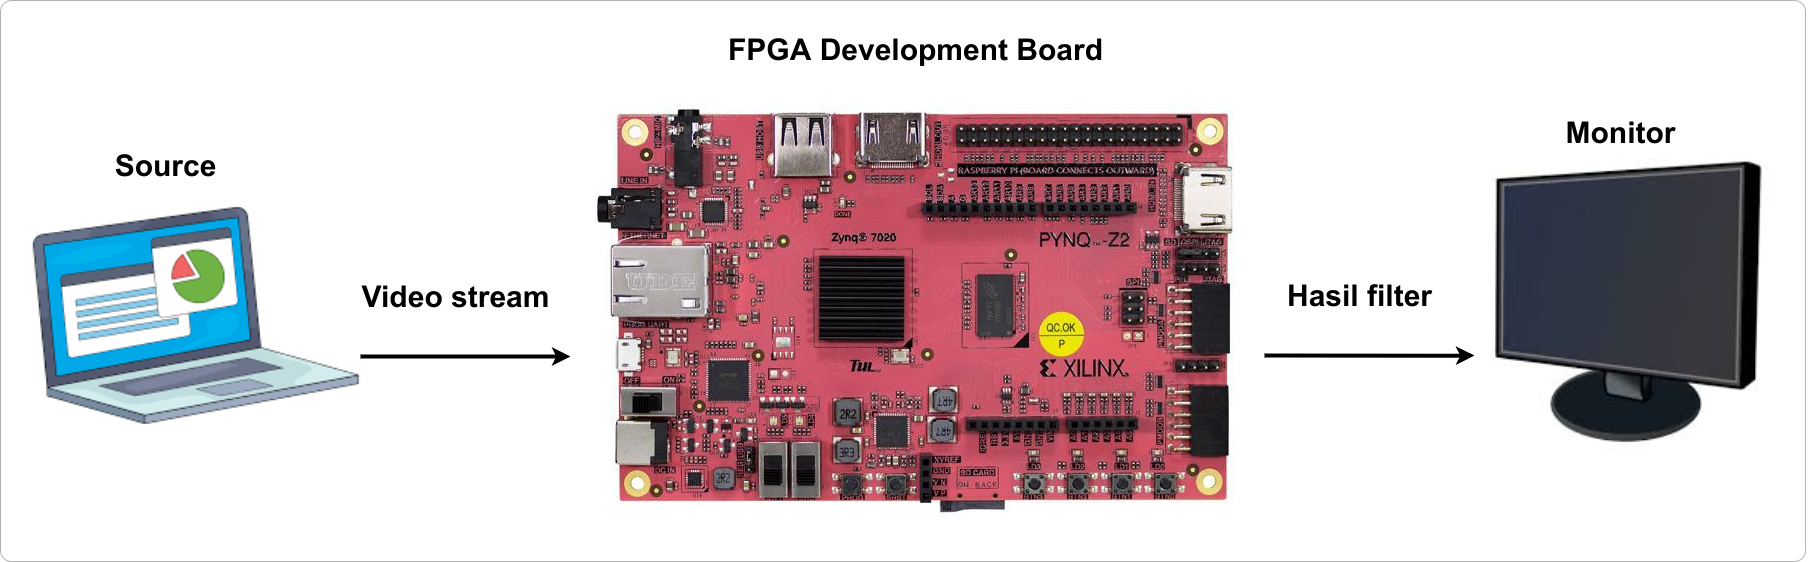
\includegraphics[width=1\textwidth, center]{images/rancangan-sistem2.png}
    \caption{Rancangan sistem.}
    \label{fig:rancangan-sistem}
\end{afigure}

Video \textit{stream} dari \textit{source} disalurkan melalui port HDMI Input pada FPGA Development Board, kemudian video \textit{stream} tersebut akan diolah dengan menerapkan filter spasial linear pada setiap framenya. Setiap frame yang telah diterapkan filter spasial akan dialirkan ke monitor untuk kemudian ditampilkan. Selanjutnya dilakukan analisis kinerja pada FPGA. FPGA Development Board yang digunakan dalam penelitian ini dapat diakses dengan \textit{ssh} pada port 22 atau dengan \textit{Jupyter Notebook} melalui \textit{web browser}.

\pagebreak

\section{Instrumen Penelitian}
\begin{enumerate}[topsep=0pt,itemsep=0pt,partopsep=0pt, parsep=0pt]
    \item Kebutuhan perangkat lunak:
    \begin{enumerate}[topsep=0pt,itemsep=0pt,partopsep=0pt, parsep=0pt, label={\alph*.}]
        \item Linux Ubuntu 18, sebagai OS pada FPGA Development Board.
        \item Python 3.6, dengan library OpenCV, Numpy, Pynq 5.2, dan Xilinx xfOpenCV.
        \item Jupyter Notebook pada FPGA Development Board. 
        \item Web Browser untuk mengakses Jupyter Notebook pada FPGA Development Board.
    \end{enumerate}
    \item Kebutuhan perangkat keras:
    \begin{enumerate}[topsep=0pt,itemsep=0pt,partopsep=0pt, parsep=0pt, label={\alph*.}]
        \item FPGA Development Board.
        \item Micro SD Card 16 GB, sebagai media penyimpanan OS pada FPGA Development Board.
        \item Monitor Eksternal, untuk menampilkan hasil penerapan filter spasial pada FPGA Development Board.
        \item Laptop Lenovo Ideapad 320 (sebagai \textit{source} video \textit{stream}).
    \end{enumerate}

    Spesifikasi FPGA Development Board yang digunakan:
    \begin{itemize}[topsep=0pt,itemsep=0pt,partopsep=0pt, parsep=0pt]
        \item Model : Xilinx PYNQ-Z2.
        \item Processor : Dual-Core ARM Cortex A9, 650 MHz
        \item FPGA : 1,3M reconfigurable gates
        \item Memory : 512 MB DDR3 / Flash
        \item Storage : Micro SD card slot
        \item Power : DC 7V-15V
        \item Dimension : 3,44" x 5,39" (87mm x 137mm)
    \end{itemize}
\end{enumerate}

    
\chapter{HASIL DAN PEMBAHASAN}


% Jelaskan Proses Implementasi 
\section{Implementasi pada FPGA Development Board}

Pada penelitian ini digunakan 6 kernel berbeda berukuran 3x3 untuk penerapan filter spasial linear pada video \textit{stream} 720p 60 FPS. Penerapan ini dilakukan pada FPGA Development Board dengan menggunakan prosesor ARM dan FPGA. Kemudian dilakukan analisis kinerja dari keduanya untuk menunjukkan masing-masing waktu komputasi, FPS, persentase penggunaan CPU, penggunaan \textit{memory}, \textit{resident memory} (RES), \textit{shared memory} (SHR), dan \textit{virtual memory} (VIRT) pada masing-masing kernel.

FPGA Development Board dirangkai seperti yang telah disebutkan pada Bab sebelumnya, pada gambar \ref{fig:rancangan-sistem}. HDMI Output pada FPGA dihubungkan ke monitor dan HDMI Input dihubungkan ke \textit{source} dalam hal ini laptop Lenovo Ideapad 320. FPGA Development Board juga dihubungkan ke \textit{router} menggunakan kabel UART agar dapat diakses menggunakan protokol \textit{ssh}. Selanjutnya memasang semua \textit{library} yang dibutuhkan untuk melakukan penerapan filter spasial linear pada video \textit{stream} menggunakan FPGA Development Board.

% \subsection{Representasi Video Stream sebagai Citra Digital}
% \subsection{Konversi Frame menjadi Grayscale}
\subsection{Penerapan Filter Spasial}
Setiap frame dari \textit{source} video \textit{stream} dibaca sebagai citra digital yang direpresentasikan sebagai matriks berukuran 1280x720 dengan rentang nilai keabuan pada masing-masing piksel yaitu dari 0 sampai 255. Setiap piksel pada matriks tersebut hanya memiliki satu lapis warna sebab citra yang diterima dari source adalah citra \textit{grayscale}, tidak seperti citra warna yang memiliki tiga lapis warna pada setiap pikselnya. 
% padding?

Proses filter spasial dilakukan dengan operasi konvolusi pada setiap matriks dengan kernel yang telah ditentukan sebelumnya. Operasi konvolusi ini menghasilkan matrix baru dengan ukuran 1280x720. Matriks hasil tersebut selanjutnya direpresentasikan kembali sebagai citra digital yang selanjutnya disebut sebagai hasil filter. Hasil filter dari setiap frame ini ditampilkan ke monitor melalui HDMI Output pada FPGA Development Board secara berkesinambungan sehingga tampak seperti video.

\begin{afigure}
    \includegraphics[width=0.8\linewidth, center]{images/output-image/input1-grayscale.png}
    \caption{Contoh Frame Grayscale.}
    \label{fig:input-grayscale}
\end{afigure}

Salah satu contoh frame dari \textit{source} dapat dilihat pada gambar \ref{fig:input-grayscale}. Selanjutnya dilakukan filter spasial menggunakan 6 kernel yang telah ditentukan sebelumnya.

\subsubsection{Average Blur}
Penerapan filter spasial pada frame \textit{grayscale} yang berukuran 1280x720 pixel dengan kernel \textit{average blur} (\ref{kernel:average}) yang berukuran 3x3 menghasilkan cita blur yang berukuran 1280x720. Hasil filter \textit{average blur} dapat dilihat pada gambar \ref{fig:output-averageblur}. Filter seperti ini dapat digunakan untuk mengurangi derau pada citra.
\begin{afigure}
    \includegraphics[width=0.8\linewidth, center]{images/output-image/input1-averageblur.png}
    \caption{Hasil filter Average Blur.}
    \label{fig:output-averageblur}
\end{afigure}

\subsubsection{Gaussian Blur}
Penerapan filter spasial dengan kernel \textit{gaussian blur} (\ref{kernel:gaussianblur}) yang berukuran 3x3 menghasilkan cita blur yang secara kasat mata mirip dengan filter \textit{average blur}. Namun apabila diperhatikan nilai masing-masing pixel pada gambar \ref{fig:output-gaussianblur} akan terlihat perbedaan dengan nilai masing-masing pixel pada gambar \ref{fig:output-averageblur}. Hal ini disebabkan oleh nilai bobot pada kernel \textit{gaussian blur} yang berbeda dengan kernel \textit{average blur} sehingga hasil konvolusinya juga berbeda. 
\begin{afigure}
    \includegraphics[width=0.8\linewidth, center]{images/output-image/input1-gaussianblur.png}
    \caption{Hasil filter Gaussian Blur.}
    \label{fig:output-gaussianblur}
\end{afigure}

\subsubsection{Laplacian}
Penerapan filter spasial dengan kernel \textit{laplacian} (\ref{kernel:laplacian}) menghasilkan cita biner yang hanya direpresentasikan dengan warna hitam dan putih saja, dapat dilihat pada gambar \ref{fig:output-laplacian}. Filter seperti ini dapat digunakan pada metode deteksi tepi dalam proses pengolahan citra digital.
\begin{afigure}
    \includegraphics[width=0.8\linewidth, center]{images/output-image/input1-laplacian.png}
    \caption{Hasil filter Laplacian.}
    \label{fig:output-laplacian}
\end{afigure}

\subsubsection{Sharpening}
Penerapan filter spasial dengan kernel \textit{sharpening} (\ref{kernel:sharpen}) dapat meningkatkan detail (seperti garis) pada citra, namun dapat juga dapat menimbulkan derau pada citra apabila bobot kernelnya tidak sesuai. Filter seperti ini lebih tepat digunakan untuk memperbaiki kualitas citra (dengan nilai kernel yang sesuai). Hasil filter \textit{sharpening} ini dapat dilihat pada gambar \ref{fig:output-sharpen}.
\begin{afigure}
    \includegraphics[width=0.8\linewidth, center]{images/output-image/input1-sharpen.png}
    \caption{Hasil filter Sharpening.}
    \label{fig:output-sharpen}
\end{afigure}

\subsubsection{Sobel Horizontal}
Penerapan filter spasial dengan kernel \textit{sobel horizontal} (\ref{kernel:sobel}) menghasilkan cita biner, dapat dilihat pada gambar \ref{fig:output-sobelhor}. Filter seperti lebih tepat digunakan pada metode deteksi tepi di citra yang banyak mengandung garis horizontal.
\begin{afigure}
    \includegraphics[width=0.8\linewidth, center]{images/output-image/input1-sobelhor.png}
    \caption{Hasil filter Sobel Horizontal.}
    \label{fig:output-sobelhor}
\end{afigure}

\subsubsection{Sobel Vertical}
Penerapan filter spasial dengan kernel \textit{sobel vertical} (\ref{kernel:sobel}) menghasilkan cita biner, dapat dilihat pada gambar \ref{fig:output-sobelver}. Sama halnya dengan filter \textit{sobel horizontal}, filter \textit{sobel vertical} juga dapat digunakan untuk metode deteksi tepi, terutama pada citra yang banyak mengandung garis verikal.
\begin{afigure}
    \includegraphics[width=0.8\linewidth, center]{images/output-image/input1-sobelver.png}
    \caption{Hasil filter Sobel Vertical.}
    \label{fig:output-sobelver}
\end{afigure}

\subsection{Penerapan Filter Spasial menggunakan Prosesor ARM dan FPGA}
Penerapan filter spasial menggunakan prosesor ARM dilakukan dengan menggunakan \textit{library} OpenCV dengan bahasa pemrograman Python yang dijalankan pada FPGA Development Board. Sedangkan untuk penerapan filter spasial menggunakan FPGA dilakukan dengan menggunakan \textit{library} xfOpenCV dari Xilinx. \textit{Library} xfOpenCV ini adalah library khusus yang dimodifikasi dari OpenCV sehingga proses komputasinya dapat dilakukan dengan FPGA, bukan dengan prosesor ARM yang pada FPGA Development Board ini. Lebih lanjut mengenai program yang digunakan dapat dilihat pada lampiran \textit{pynq-filter-spasial-arm} (\ref{code:filter-spasial-FPGA}) dan \textit{pynq-filter-spasial-fpga} (\ref{code:filter-spasial-ARM}).

\subsection{Proses Evaluasi Kinerja}
Pada penelitian ini proses dalam evaluasi kinerja dilakukan dalam dua tahap. Proses pertama untuk menghitung waktu komputasi dan FPS dari masing-masing kernel dengan prosesor ARM dan FPGA. Kemudian proses kedua untuk mencatat persentase penggunaan CPU dan penggunaan memory termasuk \textit{resident memory}, \textit{shared memory} dan \textit{virtual memory}. 

\subsubsection{Menghitung Waktu Komutasi dan FPS}
Pada proses ini peneliti melakukan percobaan dengan menggunakan 50 frame dan 200 frame dari \textit{source} untuk dihitung FPS dan waktu komputasinya. Percobaan dilakukan sebanyak 5 kali menggunakan 50 frame untuk masing-masing kernel pada prosesor ARM dan FPGA, dan 5 kali percobaan menggunakan 200 frame untuk masing-masing kernel. Hasil masing-masing percobaan ini dapat dilihat pada daftar lampiran (\ref{lampiran:waktu-komputasi}).

Menghitung waktu komputasi dilakukan dengan cara mencatat waktu mulai dan waktu semua frame selesai difilter pada setiap percobaan. Waktu komputasi diperoleh dari selisih antara waktu selesai dengan waktu mulai, seperti pada persamaan \ref{eq:time}. Dilakukan dengan 50 frame dan 200 frame pada masing-masing kernel dengan menggunakan prosesor ARM dan FPGA. Proses ini dilakukan dengan menggunakan \textit{library time} pada bahasa pemrograman Python, dapat dilihat pada gambar \ref{code:calculate-time}.
\begin{afigure}
    \lstinputlisting[frame=single, style=python]{images/programs/calculate-time.py}
    \caption{Menghitung waktu komputasi dengan library time di Python.}
    \label{code:calculate-time}
\end{afigure}

Hasil waktu komputasi ini dicatat dan kemudian digunakan untuk menghitung FPS dari masing-masing percobaan. Selanjutnya FPS masing-masing percobaan ini dihitung dengan menggunakan persamaan \ref{eq:fps}.

\subsubsection{Mencatat Penggunaan Memory dan CPU (Resource)}
Pada proses ini peneliti menggunakan fitur yang tersedia pada sistem operasi Linux yang berjalan di FPGA Development Board untuk membantu mencatat penggunaan CPU dan memory (\textit{resource}) pada saat proses penerapan filter spasial. Program ini menampilkan data tentang proses yang berjalan seperti ID sebuah proses, persentase memory yang digunakan oleh sebuah proses, persentase CPU yang digunakan, berapa lama sebuah proses berjalan, \textit{resident memory}, \textit{shared memory} dan \textit{virtual memory}. Contoh output program tersebut dapat dilihat pada gambar \ref{fig:top-linux}.
\begin{afigure}
    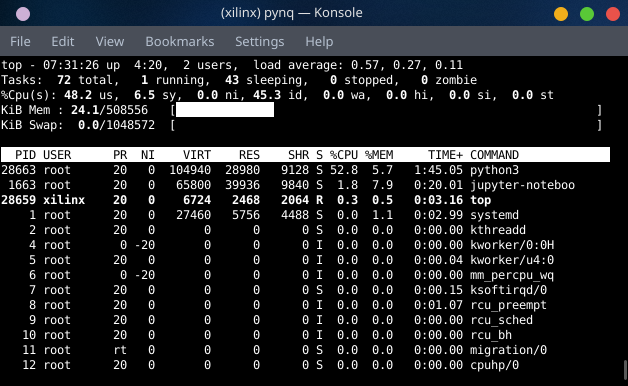
\includegraphics[width=0.8\linewidth, center]{images/programs/top-linux.png}
    \caption{Tampilan program \textbf{top}.}
    \label{fig:top-linux}
\end{afigure}

Peneliti melakukan 5 kali percobaan untuk mencatat penggunaan memory dan CPU dari masing-masing kernel dengan prosesor ARM dan FPGA. Percobaan ini dilakukan dengan menggunakan Jupyter Notebook yang berjalan pada FPGA Development Board yang dapat diakses menggunakan \textit{web browser} dari perangkat lain. Serta digunakan protokol SSH untuk mengakses FPGA Development Board dan menjalankan program untuk menampilkan penggunaan \textit{resource} dari proses yang sedang berjalan.

\begin{afigure}
    \lstinputlisting[frame=single, style=python]{images/programs/pid.py}
    \caption{Menampilkan PID sebuah proses dengan bahasa pemrograman Python.}
    \label{code:pid}
\end{afigure}

Pertama peneliti menampilkan ID proses dari Jupyter Notebook yang digunakan untuk mencatat penggunaan memory dan CPU dari penerapan filter menggunakan prosesor ARM dan FPGA. Cara menampilkan ID proses (PID) menggunakan bahasa pemrograman Python dapat dilihat pada gambar \ref{code:pid}. ID proses tersebut kemudian digunakan pada program \textbf{top} untuk menampilkan \textit{resource} yang digunakan oleh preses tersebut. 

\begin{afigure}
    \begin{lstlisting}[frame=single, style=shell] 
    $ top -d 0.1 -p 4382 -b >> arm-laplacian1.txt    
    \end{lstlisting}
    \caption{Menjalankan program \textbf{top} kemudian menyimpan hasilnya pada file arm-laplacian1.txt.}
    \label{code:top}
\end{afigure}

Pada gambar \ref{code:top} ditunjukan cara menggunakan program \textbf{top} untuk mencatat penggunaan \textit{resource} dari proses dengan ID 4382 kemudian \textit{output}nya disimpan pada file \textit{arm-laplacian1.txt}. Program \textbf{top} tersebut dijalankan sesaat sebelum proses penerapan filter dijalankan pada Jupyter Notebook. Output dari program top setiap 0.1 detik disimpan pada file text yang telah ditentukan. Setelah seluruh frame selesai difilter maka program \textbf{top} juga dihentikan.

\begin{afigure}
    \lstinputlisting[frame=single, style=plain]{images/programs/arm-laplacian1.txt}
    \caption{Potongan isi file arm-laplacian1.txt.}
    \label{code:arm-laplacian1.txt}
\end{afigure}

Isi file \textit{arm-laplacian1.txt} setelah program selesai dijalankan dapat dilihat pada gambar \ref{code:arm-laplacian1.txt}. Isi dari file hasil ini masih banyak mengandung informasi yang tidak dibutuhkan pada penelitian ini, sehingga perlu dilakukan proses ekstraksi informasi yang dibutuhkan saja. Kemudian file yang telah diekstraksi tersebut dibuat menjadi file CSV agar lebih mudah dalam proses pengolahan selanjutnya, seperti pada gambar \ref{code:arm-laplacian1.csv}. Proses tesebut dilakukan sebanyak 5 kali percobaan pada masing-masing kernel menggunakan prosesor ARM dan FPGA.

\begin{afigure}
    \lstinputlisting[frame=single, style=plain]{images/programs/arm-laplacian1.csv}
    \caption{Isi file arm-laplacian1.csv.}
    \label{code:arm-laplacian1.csv}
\end{afigure}


% Jelaskan Hasil
\section{Analisis Kinerja}
\subsection{Waktu Komuptasi}
% pengantar
% Dilakukan 5 kali percobaan dengan 50 frame dan 5 kali percobaan dengan 200 frame pada masing-masing kernel menggunakan ARM prosesor dan FPGA. 

% 50 FRAMe
Data waktu komputasi dengan menggunakan 50 frame pada maasing-masing kernel dapat dilihat pada tabel \ref{table:hasil-time50} dan grafik pada gambar \ref{fig:chart-time50}. Secara umum waktu komputasi dengan menggunakan prosesor ARM lebih lambat daripada waktu komputasi dengan menggunakan FPGA. Rata-rata waktu komputasi dengan prosesor ARM menggunakan 50 frame adalah 7,26 detik, sedangkan rata-rata waktu komputasi dengan FPGA menggunakan 50 frame hanya 0,82 detik.
\begin{atable}
    \caption{Tabel perbandingan waktu komputasi dengan menggunakan 50 frame.}
    \label{table:hasil-time50}
    \csvreader[
        head to column names,
        tabular=lcc,
        separator=semicolon,
        before table=\rowcolors{2}{gray!15}{gray!30},
        table head= \rowcolor{gray!50!black} 
            \color{white} Filter & 
            \color{white} Prosesor ARM (s) & 
            \color{white} FPGA (s)\\]
        {tables/hasil-time50.csv}
        {
            filter=\filter, 
            arm=\arm, 
            fpga=\fpga}
        {
            \filter & 
            \arm & 
            \fpga }
\end{atable}
\begin{figure}[H]
    \centering
    \includegraphics[width=0.81\linewidth, center]{images/chart/chart-time50.png}
    \caption{50 frame.}
    \label{fig:chart-time50}
    \caption{Grafik perbandingan waktu komputasi dengan 50 frame dan 200 frame}
\end{figure}

% 200 frame
Data waktu komputasi menggunakan 200 frame pada maasing-masing kernel dapat dilihat pada tabel \ref{table:hasil-time200} dan grafik pada gambar \ref{fig:chart-time200}. Rata-rata waktu komputasi dengan prosesor ARM menggunakan 200 frame adalah 29,06 detik, sedangkan rata-rata waktu komputasi dengan FPGA menggunakan 200 frame hanya 3,32 detik.
\begin{atable}
    \caption{Tabel perbandingan waktu komputasi dengan menggunakan 200 frame.}
    \label{table:hasil-time200}
    \csvreader[
        head to column names,
        tabular=lcc,
        separator=semicolon,
        before table=\rowcolors{2}{gray!15}{gray!30},
        table head= \rowcolor{gray!50!black} 
            \color{white} Filter & 
            \color{white} Prosesor ARM (s) & 
            \color{white} FPGA (s)\\]
        {tables/hasil-time200.csv}
        {
            filter=\filter, 
            arm=\arm, 
            fpga=\fpga}
        {
            \filter & 
            \arm & 
            \fpga }
\end{atable}

\begin{figure}[H]
    \centering
    \includegraphics[width=0.81\linewidth, center]{images/chart/chart-time200.png}
    \caption{200 frame.}
    \label{fig:chart-time200}
    \caption{Grafik perbandingan waktu komputasi dengan 50 frame dan 200 frame}
\end{figure}

Waktu komputasi tercepat dengan menggunakan prosesor ARM terdapat pada filter Laplacian yaitu 6,21 detik dengan 50 frame dan 24.85 detik dengan 200 frame. Sedangkan waktu komputasi paling lambat ketika menggunakan prosesor ARM terdapat pada filter Sharpening yaitu 8,04 detik dengan 50 frame dan 32,24 detik dengan 200 frame. 


\subsection{Frame Rate (FPS)}
Dengan mengetahui waktu komputasi dan jumlah frame maka frame rate atau FPS dapat dihitung menggunakan persamaan \ref{eq:fps}. Data FPS dari masing-masing kernel dengan prosesor ARM dan FPGA dapat dilihat pada tabel \ref{table:hasil-fps} dan grafik pada gambar \ref{fig:chart-fps}.
\begin{atable}
    \caption{Tabel perbandingan FPS dengan menggunakan prosesor ARM dan FPGA.}
    \label{table:hasil-fps}
    \csvreader[
        head to column names,
        tabular=lcc,
        separator=semicolon,
        before table=\rowcolors{2}{gray!15}{gray!30},
        table head= \rowcolor{gray!50!black} 
            \color{white} Filter & 
            \color{white} Prosesor ARM & 
            \color{white} FPGA\\]
        {tables/hasil-fps.csv}
        {
            filter=\filter, 
            arm=\arm, 
            fpga=\fpga}
        {
            \filter & 
            \arm & 
            \fpga }
\end{atable}
\begin{figure}[H]
    \includegraphics[width=0.81\linewidth, center]{images/chart/chart-fps.png}
    \caption{Grafik perbandingan FPS dengan menggunakan prosesor ARM dan FPGA.}
    \label{fig:chart-fps}
\end{figure}

Pada tabel \ref{table:hasil-fps} terlihat dengan menggunakan prosesor ARM diperoleh rata-rata 6.95 frame per detik (FPS), sedangkan ketika menggunakan FPGA diperoleh rata-rata 60.37 frame per detik. Terlihat pada grafik \ref{fig:chart-fps} nilai FPS dengan FPGA jauh lebih tinggi daripada dengan prosesor ARM yang ada pada FPGA Development Board.


\subsection{Penggunaan CPU}
Data perbandingan penggunaan CPU pada masing-masing kernel dengan prosesor ARM dan FPGA dapat dilihat pada tabel \ref{table:hasil-cpu} dan grafik pada gambar \ref{fig:chart-cpu}. Rata-rata penggunaan CPU dengan prosesor ARM adalah 99.58\% sedangkan dengan FPGA diperoleh 84.75\%. Data ini menunjukkan bahwa penggunaan CPU dengan prosesor ARM sedikit lebih besar daripada dengan FPGA.

\begin{atable}
    \caption{Tabel perbandingan penggunaan CPU dengan menggunakan prosesor ARM dan FPGA.}
    \label{table:hasil-cpu}
    \csvreader[
        head to column names,
        tabular=lcc,
        separator=semicolon,
        before table=\rowcolors{2}{gray!15}{gray!30},
        table head= \rowcolor{gray!50!black} 
            \color{white} Filter & 
            \color{white} Prosesor ARM (\%) & 
            \color{white} FPGA (\%)\\]
        {tables/hasil-cpu.csv}
        {
            filter=\filter, 
            arm=\arm, 
            fpga=\fpga}
        {
            \filter & 
            \arm & 
            \fpga }
\end{atable}
\begin{figure}[H]
    \includegraphics[width=0.81\linewidth, center]{images/chart/chart-cpu.png}
    \caption{Grafik perbandingan penggunaan CPU dengan menggunakan prosesor ARM dan FPGA.}
    \label{fig:chart-cpu}
\end{figure}

Penggunaan CPU terbesar dengan prosesor ARM yaitu pada kernel average blur (99,83\%) dan dengan FPGA pada kernel sobel horizontal (86,22\%). Penggunaan CPU terkecil dengan prosesor ARM yaitu pada kernel sharpening dan sobel horizontal (99,47\%) dan dengan FPGA pada kernel gaussian blur (83,70\%).


\subsection{Penggunaan Memory}
Data penggunaan memory dengan prosesor ARM dan FPGA dapat dilihat pada tabel \ref{table:hasil-mem} dan grafik pada gambar \ref{fig:chart-mem}. Data ini menunjukkan persentase memory yang digunakan pada masing-masing kernel. Rata-rata penggunaan memory dengan prosesor ARM adalah 25,37\% dan 24,86\% dengan FPGA. 
\begin{atable}
    \caption{Tabel perbandingan penggunaan memory dengan menggunakan prosesor ARM dan FPGA.}
    \label{table:hasil-mem}
    \csvreader[
        head to column names,
        tabular=lcc,
        separator=semicolon,
        before table=\rowcolors{2}{gray!15}{gray!30},
        table head= \rowcolor{gray!50!black} 
            \color{white} Filter & 
            \color{white} Prosesor ARM (\%) & 
            \color{white} FPGA (\%)\\]
        {tables/hasil-mem.csv}
        {
            filter=\filter, 
            arm=\arm, 
            fpga=\fpga}
        {
            \filter & 
            \arm & 
            \fpga }
\end{atable}
\begin{figure}[H]
    \includegraphics[width=0.81\linewidth, center]{images/chart/chart-mem.png}
    \caption{Grafik perbandingan penggunaan memory dengan menggunakan prosesor ARM dan FPGA.}
    \label{fig:chart-mem}
\end{figure}
Walaupun FPGA lebih baik daripada prosesor ARM pada segi waktu komputasi dan FPS namun penggunaan memory pada penerapan filter ini terlihat tidak jauh berbeda. Penggunaan memory FPGA ini hanya 0,51\% lebih rendah dari penggunaan memory dengan prosesor ARM.


\subsection{Resident Memory (RES)}
Data penggunaan resident memory atau RES dengan prosesor ARM dan FPGA dapat dilihat pada tabel \ref{table:hasil-res} dan grafik pada gambar \ref{fig:chart-res}. Data ini menunjukkan banyaknya RES (dalam satuan kilobyte) yang digunakan pada saat penerapan filter spasial pada video stream dengan masing-masing kernel.

\begin{atable}
    \caption{Tabel perbandingan penggunaan resident memory dengan menggunakan prosesor ARM dan FPGA.}
    \label{table:hasil-res}
    \csvreader[
        head to column names,
        tabular=lcc,
        separator=semicolon,
        before table=\rowcolors{2}{gray!15}{gray!30},
        table head= \rowcolor{gray!50!black} 
            \color{white} Filter & 
            \color{white} Prosesor ARM (KiB) & 
            \color{white} FPGA (KiB)\\]
        {tables/hasil-res.csv}
        {
            filter=\filter, 
            arm=\arm, 
            fpga=\fpga}
        {
            \filter & 
            \arm & 
            \fpga }
\end{atable}
\begin{figure}[H]
    \includegraphics[width=0.81\linewidth, center]{images/chart/chart-res.png}
    \caption{Grafik perbandingan penggunaan resident memory dengan menggunakan prosesor ARM dan FPGA.}
    \label{fig:chart-res}
\end{figure}
Rata-rata RES yang digunakan pada prosesor ARM adalah 129108,60 KiB dan 126437,20 KiB pada FPGA. Terlihat bahwa penggunaan RES pada prosesor ARM dan FPGA juga tidak jauh berbeda. Penggunaan RES terbesar dengan prosesor ARM yaitu pada kernel gaussian blur 131804,40 KiB, sedangkan dengan FPGA yaitu pada kernel sharpening 127931,20 KiB.


\subsection{Shared Memory (SHR)}
Data penggunaan shared memory dengan prosesor ARM dan FPGA dapat dilihat pada tabel \ref{table:hasil-shr} dan grafik pada gambar \ref{fig:chart-shr}. Data ini menunjukkan banyaknya shared memory (dalam satuan kilobyte) yang digunakan pada saat penerapan filter spasial pada video stream dengan masing-masing kernel.
\begin{atable}
    \caption{Tabel perbandingan penggunaan shared memory dengan menggunakan prosesor ARM dan FPGA.}
    \label{table:hasil-shr}
    \csvreader[
        head to column names,
        tabular=lcc,
        separator=semicolon,
        before table=\rowcolors{2}{gray!15}{gray!30},
        table head= \rowcolor{gray!50!black} 
            \color{white} Filter & 
            \color{white} Prosesor ARM (KiB) & 
            \color{white} FPGA (KiB)\\]
        {tables/hasil-shr.csv}
        {
            filter=\filter, 
            arm=\arm, 
            fpga=\fpga}
        {
            \filter & 
            \arm & 
            \fpga }
\end{atable}
\begin{figure}[H]
    \includegraphics[width=0.81\linewidth, center]{images/chart/chart-shr.png}
    \caption{Grafik perbandingan penggunaan shared memory dengan menggunakan prosesor ARM dan FPGA.}
    \label{fig:chart-shr}
\end{figure}
Rata-rata penggunaan shared memory pada prosesor ARM adalah 56325,57 KiB dan 54030,80 KiB pada FPGA. Terlihat bahwa penggunaan shared memory pada prosesor ARM sedikit lebih besar daripada FPGA. Penggunaan shared memory terbesar pada prosesor ARM yaitu pada kernel gaussian blur 56503,60 KiB dan kernel laplacian 55528,80 KiB pada FPGA. Penggunaan shared memory terkecil pada prosesor ARM yaitu pada kernel average blur 56157,40 KiB dan kernel laplacian 42568 KiB pada FPGA.

\subsection{Virtual Memory (VIRT)}
Data penggunaan virtual memory atau VIRT dapat dilihat pada tabel \ref{table:hasil-virt} dan grafik pada gambar \ref{fig:chart-virt}. Data ini menunjukkan banyaknya virtual memory (dalam satuan kilobyte) yang digunakan pada saat penerapan filter spasial pada video stream dengan masing-masing kernel.
\begin{atable}
    \caption{Tabel perbandingan penggunaan virtual memory dengan menggunakan prosesor ARM dan FPGA.}
    \label{table:hasil-virt}
    \csvreader[
        head to column names,
        tabular=lcc,
        separator=semicolon,
        before table=\rowcolors{2}{gray!15}{gray!30},
        table head= \rowcolor{gray!50!black} 
            \color{white} Filter & 
            \color{white} Prosesor ARM (KiB) & 
            \color{white} FPGA (KiB)\\]
        {tables/hasil-virt.csv}
        {
            filter=\filter, 
            arm=\arm, 
            fpga=\fpga}
        {
            \filter & 
            \arm & 
            \fpga }
\end{atable}
\begin{figure}[H]
    \includegraphics[width=0.81\linewidth, center]{images/chart/chart-virt.png}
    \caption{Grafik perbandingan penggunaan virtual memory dengan menggunakan prosesor ARM dan FPGA.}
    \label{fig:chart-virt}
\end{figure}
Rata-rata penggunaan VIRT pada prosesor ARM adalah 395407,64 KiB dan 395501,33 KiB pada FPGA. Rata-rata penggunaan VIRT pada FPGA sedikit lebih tinggi dari pada prosesor ARM. Penggunaan VIRT terbesar pada prosesor ARM yaitu pada kernel gaussian blur 398862,80 KiB dan kernel laplacian 395638,40 KiB. Penggunaan VIRT terkecil pada prosesor ARM yaitu pada kernel 393544,80 KiB dan kernel sobel vertical 395385,60 KiB pada FPGA.

    
\chapter{KESIMPULAN DAN SARAN}

\section{Kesimpulan}
Berdasarkan hasil penerapan filter spasial linear pada FPGA Development Board dengan menggunakan 6 kernel, peneliti dapat menarik beberapa kesimpulan sebagai berikut:
\begin{enumerate}[topsep=0pt,itemsep=0pt,partopsep=0pt, parsep=0pt]
    \item Proses implementasi
    \item Waktu komputasi dan FPS dengan menggunakan FPGA secara umum lebih baik dibandingkan dengan menggunaan prosesor ARM. Penggunaan CPU pada FPGA sedikit lebih rendah dibandingkan penggunaan CPU pada prosesor ARM. Secara umum penggunaan memory, shared memory, virtual memory, dan resident memory pada FPGA tidak jauh berbeda dengan yang digunakan pada prosesor ARM.
\end{enumerate}


\section{Saran}
Setelah melakukan penelitian ini, peneliti dapat memberikan beberapa saran sebagai berikut:
\begin{enumerate}[topsep=0pt,itemsep=0pt,partopsep=0pt, parsep=0pt]
    \item Pada penelitian ini peneliti hanya menggunakan 6 kernel dengan ukuran 3x3 yaitu average blur, gaussian blur, laplacian, sharpening, sobel horizontal dan sobel vertical. Untuk kedepannya, disarankan untuk menggunakan kernel lain dengan ukuran yang lebih beragam.
    \item Pada penelitian ini peneliti hanya menggunakan metode pemrosesan citra low-level yaitu filter spasial linear, kedepannya disarankan menggunakan metode pemrosesan citra mid-level atau pemrosesan high-level.
    \item Melakukan pengolahan citra digital pada jenis citra warna, tidak terbatas hanya pada citra grayscale saja.
\end{enumerate}
    %-----------------------------------------------------------------------------
    % End Daftar masukan untuk Bab
    %=============================================================================

    %=============================================================================
    % Daftar Pustaka
    %-----------------------------------------------------------------------------
    \addcontentsline{toc}{chapter}{DAFTAR PUSTAKA}
    \printbibliography[title={DAFTAR PUSTAKA}]
    %-----------------------------------------------------------------------------
    % End Daftar Pustaka
    %=============================================================================
    
    \addcontentsline{toc}{chapter}{LAMPIRAN}
    \addtocontents{toc}{\protect\setcounter{tocdepth}{0}}
    \chapter*{LAMPIRAN}
\setcounter{chapter}{7}

\section{Data Hasil Percobaan ARM Average Blur}

\subsection{Percobaan 1}
% ARM Average Blur Percobaan 1    
\csvautolongtable[separator=semicolon]{tables/performance-test/arm-aveblur1.csv}

\subsection{Percobaan 2}
% ARM Average Blur Percobaan 2    
\csvautolongtable[separator=semicolon]{tables/performance-test/arm-aveblur2.csv}

\subsection{Percobaan 3}
% ARM Average Blur Percobaan 3    
\csvautolongtable[separator=semicolon]{tables/performance-test/arm-aveblur3.csv}

\subsection{Percobaan 4}
% ARM Average Blur Percobaan 4    
\csvautolongtable[separator=semicolon]{tables/performance-test/arm-aveblur4.csv}

\subsection{Percobaan 5}
% ARM Average Blur Percobaan 5    
\csvautolongtable[separator=semicolon]{tables/performance-test/arm-aveblur5.csv}

% \begin{table}
%     \renewcommand{\arraystretch}{1.5} 
%     \caption{ARM Average Blur Percobaan 1}
%     \label{table:arm-aveblur1}
%     \csvreader[
%         % column count = 11,
%         head to column names,
%         longtable=cccccccc,
%         separator=semicolon,
%         late after line=\\,
%         before table=\rowcolors{2}{gray!15}{gray!30},
%         table head= \rowcolor{gray!50!black} 
%             \color{white} PID & 
%             \color{white} VIRT & 
%             \color{white} RES &
%             \color{white} SHR & 
%             \color{white} Status &  
%             \color{white} CPU(\%) &
%             \color{white} MEM(\%) & 
%             \color{white} Time(s) 
%             \\]
%         {tables/performance-test/arm-aveblur2.csv}
%         {
%             PID=\PID, 
%             VIRT=\VIRT, 
%             RES=\RES,
%             SHR=\SHR, 
%             S=\S,
%             CPU=\CPU,
%             MEM=\MEM, 
%             TIME=\TIME}
%         {
%             \PID & 
%             \VIRT & 
%             \RES &
%             \SHR & 
%             \S &
%             \CPU &
%             \MEM & 
%             \TIME}
% \end{table}


\end{document}
